\documentclass{beamer}

% packages
\usepackage{graphicx}
\usepackage{enumitem}

% metadata
\title{ECE 453 Project Proposal}
\author{Vaughn Kottler}
\author{Mayank Katwal}
\author{Cooper Green}
\date{\today}

\begin{document}

% title slide
\begin{frame}
\begin{center}
{\Large\textbf{Fault-Tolerant Quadcopter}}\\
\vspace{\baselineskip}
ECE 453 Project Proposal (Fall 2018)\\
University of Wisconsin-Madison\\
\vspace{\baselineskip}
{\large\textit{Vaughn Kottler, Mayank Katwal, Cooper Green}}
\end{center}
\end{frame}

% top-level block diagram
\begin{frame}
\frametitle{Overview}
\begin{center}
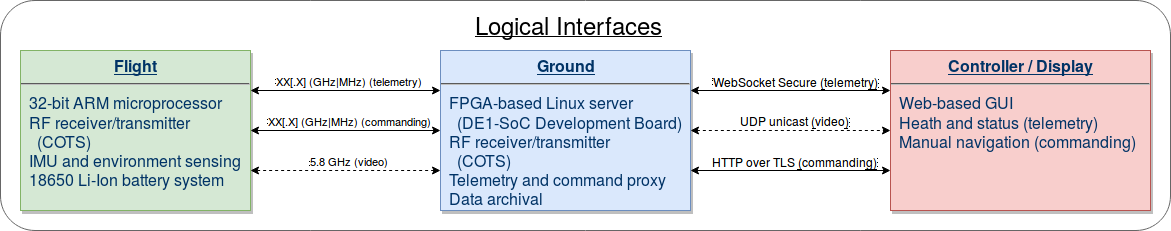
\includegraphics[width=\linewidth]{../src/im/top_level}
\end{center}
\vspace{\baselineskip}
\begin{description}[align=right,labelwidth=80pt,itemsep=10pt]
\item [Quadcopter] -- Battery-powered, four-motor flying machine
\item [Ground Station] -- Linux server managing the quadcopter's
	radio endpoint, hosts wired-network services (i.e.\ telemetry)
\item [Web-based UI] -- A modern dashboard for visualizing data
	and manually commanding the vehicle
\end{description}
\end{frame}

% learning objectives and features
\begin{frame}
\frametitle{Learning Objectives and Features}
Exposure to:
\begin{itemize}
	\item [--] Radio-frequency communication
	\item [--] Control theory
	\item [--] SoC platform(s)
	\item [--] Data pipelining in the aerospace/avionics problem space
	\item [--] Modern user-interface design and implementation
\end{itemize}
\vspace{\baselineskip}
Features:
\begin{description}[align=right,labelwidth=120pt]
	\item [Single-Fault Tolerant] -- Land safely in the event of communication
		``heartbeat timeout''
	\item [Telemetry Archival] -- Implement long-term telemetry storage for
		post-flight data analysis
\end{description}
\end{frame}

% quadcopter
\begin{frame}
\frametitle{Quadcopter}
\begin{center}
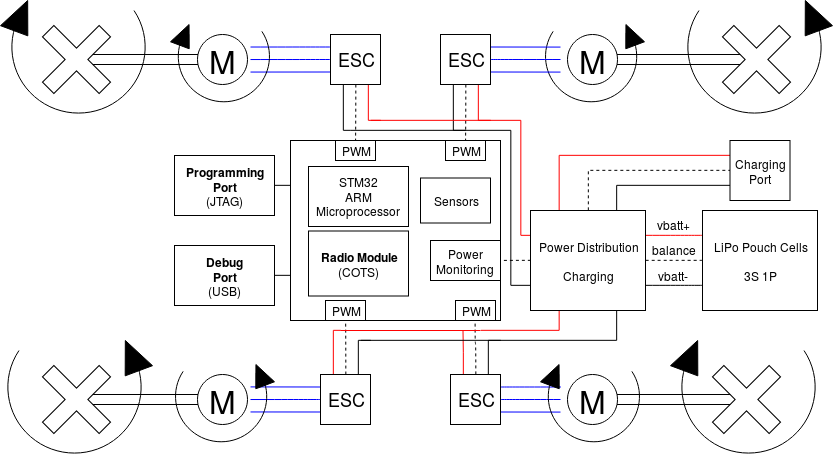
\includegraphics[width=\linewidth]{../src/im/quadcopter}
\end{center}
\end{frame}

% ground station
\begin{frame}
\frametitle{Ground Station}
\begin{center}
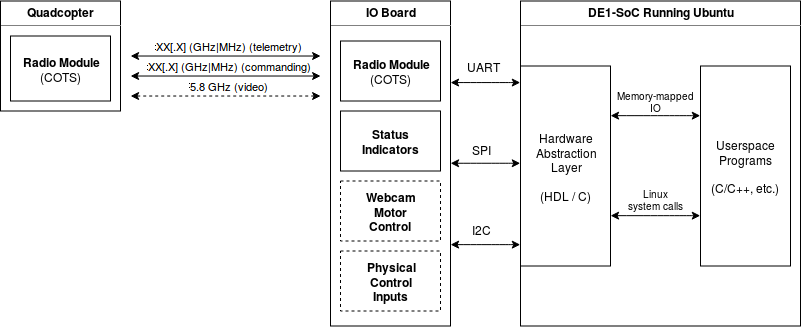
\includegraphics[width=\linewidth]{../src/im/ground_station}
\end{center}
\end{frame}

% display and controller
\begin{frame}
\frametitle{User Interface}
\begin{center}
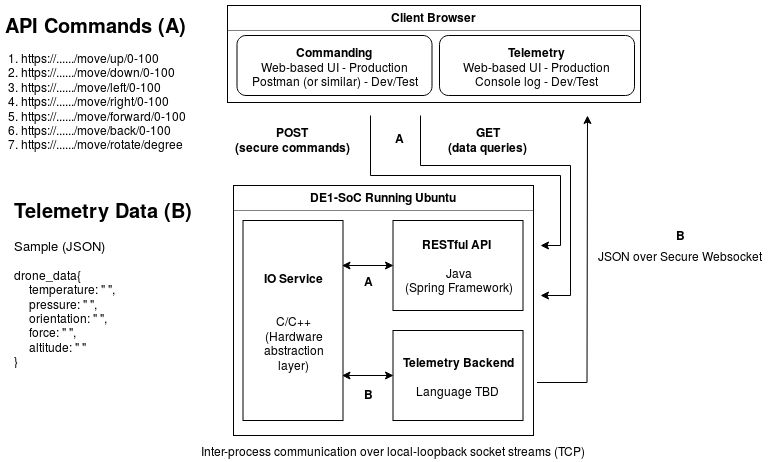
\includegraphics[height=225pt,width=\linewidth,keepaspectratio]{../src/im/display_controller}
\end{center}
\end{frame}

\end{document}
